\documentclass[11pt]{article}

%% PACKAGES
\usepackage{graphicx}
\usepackage{verbatim}
\usepackage{url}
\usepackage[printonlyused]{acronym}
\usepackage[ruled]{algorithm}
\usepackage{amsmath,amssymb,amsfonts,amsthm}
\usepackage{overpic}
\usepackage{calc}
\usepackage{color,soul}
%\usepackage{times}
%\usepackage{ragged2e}
 \usepackage[margin=1.0in]{geometry}
\usepackage[colorlinks=false]{hyperref}
\usepackage{textcomp}
\usepackage{cite}
\usepackage{mdwlist}
\usepackage{subfiles}
\usepackage{enumitem}
\usepackage{calc}
\usepackage{array}
\usepackage{units}
\usepackage{arydshln,leftidx,mathtools}
\usepackage[caption=false,font=footnotesize]{subfig}
\usepackage{relsize}
\usepackage{float}
\usepackage{makecell}

\usepackage{algorithm}
\usepackage[noend]{algpseudocode}

\usepackage{listings}
\lstset{basicstyle=\small\ttfamily,columns=flexible,breaklines=true,xleftmargin=-0.5in,keepspaces=true}

\usepackage{tabularx}

\makeatletter
\let\@tmp\@xfloat
\usepackage{fixltx2e}
\let\@xfloat\@tmp
\makeatother

\usepackage[subfigure]{tocloft}
\usepackage[singlespacing]{setspace}
%\usepackage[nodisplayskipstretch]{setspace}
%\setstretch{1.0}

%\renewcommand\cftsecafterpnum{\vskip\baselineskip}
%\renewcommand\cftsubsecafterpnum{\vskip\baselineskip}
%\renewcommand\cftsubsubsecafterpnum{\vskip\baselineskip}

%\usepackage{mathtools}
%\usepackage[framed]{mcode}

\usepackage{pgfplots}

\usepackage{cancel}

\usepackage{tikz}
\usetikzlibrary{calc,patterns,decorations.pathmorphing,decorations.markings,fit,backgrounds}

\usepackage[strict]{changepage} %use to manually place figs/tables to get them within the margins

\makeatletter
\g@addto@macro\normalsize{%
  \setlength\abovedisplayskip{0.25pt}
  \setlength\belowdisplayskip{0.25pt}
  \setlength\abovedisplayshortskip{0.25pt}
  \setlength\belowdisplayshortskip{0.25pt}
}
\makeatother



\setlength{\parskip}{\baselineskip}

%% GRAPHICS PATH
\graphicspath{{../../../shared_latex_inputs/images}{../../../shared_latex_inputs/graphs}}

%% TODO
\newcommand{\todo}[1]{\vspace{5 mm}\par \noindent \framebox{\begin{minipage}[c]{0.98 \columnwidth} \ttfamily\flushleft \textcolor{red}{#1}\end{minipage}}\vspace{5 mm}\par}

%% MACROS
\providecommand{\abs}[1]{\lvert#1\rvert}
\providecommand{\norm}[1]{\lVert#1\rVert}
\providecommand{\dualnorm}[1]{\norm{#1}_\ast}
\providecommand{\set}[1]{\lbrace\,#1\,\rbrace}
\providecommand{\cset}[2]{\lbrace\,{#1}\nobreak\mid\nobreak{#2}\,\rbrace}
\providecommand{\onevect}{\mathbf{1}}
\providecommand{\zerovect}{\mathbf{0}}
\providecommand{\field}[1]{\mathbb{#1}}
\providecommand{\C}{\field{C}}
\providecommand{\R}{\field{R}}
\providecommand{\polar}{\triangle}
\providecommand{\Cspace}{\mathcal{Q}}
\providecommand{\Fspace}{\mathcal{F}}
\providecommand{\free}{\text{\{}\mathsf{free}\text{\}}}
\providecommand{\iff}{\Leftrightarrow}
\providecommand{\qstart}{q_\text{initial}}
\providecommand{\qgoal}{q_\text{final}}
\providecommand{\contact}[1]{\Cspace_{#1}}
\providecommand{\feasible}[1]{\Fspace_{#1}}
\providecommand{\prob}[2]{p(#1|#2)}
\providecommand{\prior}[1]{p(#1)}
\providecommand{\Prob}[2]{P(#1|#2)}
\providecommand{\Prior}[1]{P(#1)}
\providecommand{\parenth}[1] {\left(#1\right)}
\providecommand{\braces}[1] {\left\{#1\right\}}
\providecommand{\micron}{\hbox{\textmu m}}

%% MATH FUNCTION NAMES
\DeclareMathOperator{\conv}{conv}
\DeclareMathOperator{\cone}{cone}
\DeclareMathOperator{\homog}{homog}
\DeclareMathOperator{\domain}{dom}
\DeclareMathOperator{\range}{range}
\DeclareMathOperator{\argmax}{arg\,max}
\DeclareMathOperator{\argmin}{arg\,min}
\DeclareMathOperator{\area}{area}
\DeclareMathOperator{\sign}{sign}
\DeclareMathOperator{\mathspan}{span}
\DeclareMathOperator{\sn}{sn}
\DeclareMathOperator{\cn}{cn}
\DeclareMathOperator{\dn}{dn}
\DeclareMathOperator*{\minimize}{minimize}

\DeclareMathOperator{\atan2}{atan2}

\newtheorem{theorem}{Theorem}
\newtheorem{lemma}[theorem]{Lemma}

%\setlength{\RaggedRightParindent}{2em}
%\setlength{\RaggedRightRightskip}{0pt plus 3em}
%\pagestyle{empty}

\newcommand{\acposs}[1]{%
	\expandafter\ifx\csname AC@#1\endcsname\AC@used
	\acs{#1}'s%
	\else
	\aclu{#1}'s (\acs{#1}'s)%
	\fi
}


\title{{\Huge EMTGv9 Windows Build Guide}}
\vspace{0.5cm}
\author
{
	Noble Hatten\thanks{Aerospace Engineer, NASA Goddard Space Flight Center, Code 595}
	Edwin Dove\thanks{Aerospace Engineer, NASA Goddard Space Flight Center, Code 595}
	Tim Sullivan \thanks{Aerospace Engineer, The Aerospace Corporation}
}
\vspace{0.5cm}

\date{}

\begin{document}

\begin{titlepage}
\maketitle
%\thispagestyle{empty}
\begin{table}[H]
	\centering
	\begin{tabularx}{\textwidth}{|l|l|X|}
		\hline
		\textbf{Revision Date} & \textbf{Author} & \textbf{Description of Change} \\ \hline
		\date{January 10, 2023} & Edwin Dove & Created public release version of windows install guide.\\	\hline
		\date{January 19, 2023} & Noble Hatten & Edits to Edwin Dove's initial draft.\\	\hline
		\date{March 8, 2023} & \makecell{Tim Sullivan and \\ Edwin Dove} & Added SNOPT compile instructions and image captions.\\	\hline
		\date{July 14, 2023} & Tim Sullivan & Added updates for SNOPT 7.7.\\	 \hline
	\end{tabularx}
\end{table}
\end{titlepage}

\newpage
\tableofcontents
\thispagestyle{empty}
\newpage

\clearpage
\setcounter{page}{1}




\section*{List of Acronyms}
\begin{acronym}
%To define the acronym and include it in the list of acronyms: \acro{acronym}{definition}
%To define the acronym and exclude it from the list of acronyms:  \acro{acronym}{definition}
%
%\ac{acronym} Expand and identify the acronym the first time; use only the acronym thereafter
%\acf{acronym} Use the full name of the acronym.
%\{acronym} Use the acronym, even before the first corresponding \ac command
%\acl{acronym}  Expand the acronym without using the acronym itself.
%
%

\acro{ACS}{attitude control system}
\acro{ACO}{Ant Colony Optimization}
\acro{AD}{Automatic Differentiation}
\acro{ADL}{Architecture Design Laboratory}
\acro{AES}{Advanced Exploration Systems}
\acro{AGA}{aerogravity assist}
\acro{ALARA}{As Low As Reasonably Achievable}
\acro{API}{application programming interface}
\acro{BB}{branch and bound}
\acro{BVP}{Boundary Value Problem}
\acro{CATO}{Computer Algorithm for Trajectory Optimization}
\acro{CL}{confidence level}
\acro{CONOPS}{concept of operations}
\acro{COV}{Calculus of Variations}
\acro{D/AV}{Descent/Ascent Vehicle}
\acro{DE}{Differential Evolution}
\acro{DLA}{Declination of Launch Asymptote}
\acro{RLA}{Right Ascension of Launch Asymptote}
\acro{RA}{right ascension}
\acro{DEC}{declination}
\acro{DPTRAJ/ODP}{Double Precision Trajectory and Orbit Determination Program}
\acro{DSH}{Deep Space Habitat}
\acro{DSN}{Deep Space Network}
\acro{DSMPGA}{Dynamic-Size Multiple Population Genetic Algorithm}
\acro{EB}{Evolutionary Branching}
\acro{ECLSS}{environmental control and life support system}
\acro{ELV}{expendable launch vehicle}
\acro{EMME}{Earth to Mars, Mars to Earth}
\acro{EMMVE}{Earth to Mars, Mars to Venus to Earth}
\acro{EMTG}{Evolutionary Mission Trajectory Generator}
\acro{EVMME}{Earth to Venus to Mars, Mars to Earth}
\acro{EVMMVE}{Earth to Venus to Mars, Mars to Venus to Earth}
\acro{ERRV}{Earth Return Re-entry Vehicle}
\acro{FISO}{Future In-Space Operations}
\acro{FMT}{Fast Mars Transfer}
\acro{GASP}{Gravity Assist Space Pruning}
\acro{GCR}{galactic cosmic radiation}
\acro{GRASP}{Greedy Randomized Adaptive Search Procedure}
\acro{GSFC}{Goddard Space Flight Center}
\acro{GTOC}{Global Trajectory Optimization Competition}
\acro{GTOP}{Global Trajectory Optimization Problem}
\acro{HAT}{Human Architecture Team}
\acro{HGGA}{Hidden Genes Genetic Algorithm}
\acro{IMLEO}{Initial Mass in \acl{LEO}}
\acro{IPOPT}{Interior Point OPTimizer}
\acro{ISS}{International Space Station}
\acro{JHUAPL}{Johns Hopkins University Applied Physics Laboratory}
\acro{JSC}{Johnson Space Center}
\acro{KKT}{Karush-Kuhn-Tucker}
\acro{LEO}{Low Earth Orbit}
\acro{LRTS}{lazy race tree search}
\acro{MONTE}{Mission analysis, Operations, and Navigation Toolkit Environment}
\acro{MCTS}{Monte Carlo tree search}
\acro{MGA}{Multiple Gravity Assist}
\acro{MIRAGE}{Multiple Interferometric Ranging Analysis using GPS Ensemble}
\acro{MOGA}{Multi-Objective Genetic Algorithm}
\acro{MOSES}{Multiple Orbit Satellite Encounter Software}
\acro{MPI}{message passing interface}
\acro{MPLM}{Multi-Purpose Logistics Module}
\acro{MSFC}{Marshall Space Flight Center}
\acro{NELLS}{NASA Exhaustive Lambert Lattice Search}
\acro{NSGA}{Non-Dominated Sorting Genetic Algorithm}
\acro{NSGA-II}{Non-Dominated Sorting Genetic Algorithm II}
\acro{NHATS}{Near-Earth Object Human Space Flight Accessible Targets Study}
\acro{NTP}{Nuclear Thermal Propulsion}
\acro{OD}{orbit determination}
\acro{OOS}{On-Orbit Staging}
\acro{PCC}{Pork Chop Contour}
\acro{PEL}{permissible exposure limits}
\acro{PLATO}{PLAnetary Trajectory Optimization}
\acro{REID}{risk of exposure-induced death}
\acro{RTBP}{Restricted Three Body Problem}
\acro{SA}{Simulated Annealing}
\acro{SLS}{Space Launch System}
\acro{SNOPT}{Sparse Nonlinear OPTimizer}
\acro{SOI}{sphere of influence}
\acro{SPE}{solar particle events}
\acro{SQP}{sequential quadratic programming}
\acro{SRAG}{Space Radiation Analysis Group}
\acro{TEI}{Trans-Earth Injection}
\acro{TOF}{time of flight}
\acro{TPBVP}{Two Point Boundary Value Problem}
\acro{TMI}{Trans-Mars Injection}
\acro{VARITOP}{Variational calculus Trajectory Optimization Program}
\acro{VILM}{v-infinity leveraging maneuver}
\acro{MOI}{Mar Orbit Injection}
\acro{PCM}{Pressurized Cargo Module}
\acro{STS}{Space Transportation System}
\acro{EDS}{Earth Departure Stage}
\acro{NEO}{near-Earth asteroid}
\acro{IDC}{Integrated Design Center}
\acro{SEP}{solar-electric propulsion}
\acro{SRP}{solar radiation pressure}
\acro{NEP}{nuclear-electric propulsion}
\acro{REP}{radioisotope-electric propulsion}
\acro{DRM}{Design Reference Missions}

\acro{EDL}{entry, descent, and landing}
\acro{ASCII}{American Standard Code for Information Interchange}
\acro{AU}{Astronomical Unit}
\acro{BWG}{Beam Waveguides}
\acro{CCB}{Configuration Control Board}
\acro{CMO}{Configuration Management Office}
\acro{CODATA}{Committee on Data for Science and Technology}
\acro{DEEVE}{Dynamically Equivalent Equal Volume Ellipsoid}
\acro{DRA}{Design Reference Asteroid}
\acro{EME2000}{Earth Centered, Earth Mean Equator and Equinox of J2000 (Coordinate Frame)}
\acro{EOP}{Earth Orientation Parameters}
\acro{ET}{Ephemeris Time}
\acro{FDS}{Flight Dynamics System}
\acro{FTP}{File Transfer Protocol}
\acro{GSFC}{Goddard Space Flight Center}
\acro{PI}{Principal Investigator}
\acro{HEF}{High Efficiency}
\acro{IAG}{International Association of Geodesy}
\acro{IAU}{International Astronomical Union}
\acro{IERS}{International Earth Rotation and Reference Systems Service}
\acro{ICRF}{International Celestial Reference Frame}
\acro{ITRF}{International Terrestrial Reference System}
\acro{IOM}{Interoffice Memorandum}
\acro{JD}{Julian Date}
\acro{JPL}{Jet Propulsion Laboratory}
\acro{LM}{Lockheed Martin}
%\acro{LP150Q}{}
%\acros{LP100K}{}
\acro{MAVEN}{Mars Atmosphere and Volatile EvolutioN}
\acro{MJD}{Modified Julian Date}
\acro{MOID}{Minimum Orbit Intersection Distance}
\acro{MPC}{Minor Planet Center}
\acro{NASA}{National Aeronautics and Space Administration}
\acro{NDOSL}{\ac{NASA} Directory of Station Locations}
\acro{NEA}{near-Earth asteroid}
\acro{NEO}{near-Earth object}
\acro{NIO}{Nav IO}
\acro{OSIRIS-REx}{Origins Spectral Interpretation Resource Identification Security-Regolith Explorer}
\acro{PHA}{Potentially Hazardous Asteroid}
\acro{PHO}{Potentially Hazardous Object}
\acro{SBDB}{Small-Body Database}
\acro{SI}{International System of Units}
\acro{SPICE}{Spacecraft Planet Instrument Camera-matrix Events}
\acro{SPK}{SPICE Kernel}
\acro{SRC}{Sample Return Capsule}
\acro{SSD}{Solar System Dynamics}
\acro{STK}{Systems Tool Kit}
\acro{TAI}{International Atomic Time}
\acro{TBD}{To Be Determined}
\acro{TBR}{To Be Reviewed}
\acro{TCB}{Barycentric Coordinate Time}
\acro{TDB}{Temps Dynamiques Barycentrique, Barycentric Dynamical Time}
\acro{TDT}{Terrestrial Dynamical Time}
\acro{TT}{Terrestrial Time}
\acro{URL}{Uniform Resource Locator}
\acro{UT}{Universal Time}
\acro{UT1}{Universal Time Corrected for Polar Motion}
\acro{UTC}{Coordinated Universal Time}
\acro{USNO}{U. S. Naval Observatory}
\acro{YORP}{Yarkovsky-O'Keefe-Radzievskii-Paddack}

\acro{NLP}{nonlinear program}
\acro{MBH}{monotonic basin hopping}
\acro{MBH-C}{monotonic basin hopping with Cauchy hops}
\acro{FBS}{forward-backward shooting}
\acro{MGALT}{Multiple Gravity Assist with Low-Thrust}
\acro{MGALTS}{Multiple Gravity Assist with Low-Thrust using the Sundman transformation}
\acro{MGA-1DSM}{Multiple Gravity Assist with One Deep Space Maneuver}
\acro{MGAnDSMs}{Multiple Gravity Assist with \textit{n} Deep-Space Maneuvers using Shooting}
\acro{PSFB}{Parallel Shooting with Finite-Burn}
\acro{PSBI}{Parallel Shooting with Bounded Impulses}
\acro{FBLT}{Finite-Burn Low-Thrust}
\acro{FBLTS}{Finite-Burn Low-Thrust using the Sundman transformation}
\acro{ESA}{European Space Agency}
\acro{ACT}{Advanced Concepts Team}
\acro{IRAD}{independent research and development}
\acro{Isp}[$\text{I}_{sp}$]{specific impulse}
\acro{C3}[$C_3$]{hyperbolic excess energy}
\acro{GA}{genetic algorithm}
\acro{GALLOP}{ Gravity Assisted Low-thrust Local Optimization Program}
\acro{MALTO}{Mission Analysis Low-Thrust Optimization}
\acro{PaGMO}{Parallel Global Multiobjective Optimizer}
\acro{FRA}{feasible region analysis}
\acro{CP}{conditional penalty}
\acro{HOC}{hybrid optimal control}
\acro{HOCP}{hybrid optimal control problem}
\acro{PSO}{particle swarm optimization}
\acro{SEPTOP}{Solar Electric Propulsion Trajectory Optimization Program}
\acro{STOUR}{Satellite Tour Design Program}
\acro{STOUR-LTGA}{Satellite Tour Design Program - Low Thrust, Gravity Assist}
\acro{PaGMO}{Parallel Global Multiobjective Optimizer}
\acro{SDC}{static/dynamic control}
\acro{DDP}{Differential Dynamic Programming}
\acro{HDDP}{Hybrid Differential Dynamic Programming}
\acro{ACT}{Advanced Concepts Team}
\acro{GMAT}{General Mission Analysis Toolkit}
\acro{BOL}{beginning of life}
\acro{EOL}{end of life}
\acro{KSC}{Kennedy Space Center}
\acro{VSI}{variable \ac{Isp}}
\acro{RTG}{radioisotope thermal generator}
\acro{ASRG}{advanced Stirling radiosotope generator}
\acro{ARRM}{Asteroid Robotic Redirect Mission}
\acro{AATS}{Alternative Architecture Trade Study}
\acro{PPU}{power processing unit}
\acro{STM}{state transition matrix}
\acro{MTM}{maneuver transition matrix}
\acro{HPTM}{half-phase transition matrix}
\acro{BCI}{body-centered inertial}
\acro{BCF}{body-centered fixed}
\acro{UTTR}{Utah Test and Training Range}
\acro{EPV}{equatorial projection of $\mathbf{v}_\infty$}
\acro{KBO}{Kuiper belt object}
\acro{DSM}{deep-space maneuver}
\acro{BPT}{body-probe-thrust}
\acro{4PL}{four parameter logistic}
\acro{BCF}{body-centered fixed}
\acro{COE}{classical orbit elements}
\acro{GSL}{Gnu Scientific Library}
\acro{NEXT}{NASA's Evolutionary Xenon Thruster}

\acro{SMA}{semi-major axis}
\acro{ECC}{eccentricity}

\acro{GSAD}{Ghosh Sparse Algorithmic Differentiation}

\end{acronym}

% --------------------------------------------------------------------------------------------------------------------------
% --------------------------------------------------------------------------------------------------------------------------


%%%%%%%%%%%%%%%%%%%%%%%%
\section{Introduction}
\label{sec:introduction}
%%%%%%%%%%%%%%%%%%%%%%%%

The purpose of this document is to describe:

\begin{itemize}
	\item How to obtain the \ac{EMTG} codebase using the public NASA GitHub Repository (Section~\ref{sec:obtaining_emtg}).
	\item How to obtain the dependencies of \ac{EMTG} (Sections~\ref{sec:install_prerequisites} and~\ref{sec:obtaining_dependencies}).
	\item How to compile \ac{EMTG} from source on a Windows system (Section~\ref{sec:building_emtg}).
\end{itemize}

\noindent As may be inferred from the first bullet above, the target audience of this document is the public.

Other notes about the contents of this document:

\begin{itemize}
	\item When listing \acposs{EMTG} dependencies, specific versions of the dependencies are listed. These dependencies are known to work. The use of other versions of dependencies is not guaranteed to work and is not recommended.
	\item The instructions in this document are intended to be followed in the order in which they are given.
\end{itemize}

%%%%%%%%%%%%%%%%%%%%%%%%
\section{EMTG Prerequisites}
\label{sec:install_prerequisites}
%%%%%%%%%%%%%%%%%%%%%%%%

%%%%%%%%%%%%%%%%%%%%%%%%
% EMTG Prerequisites
%%%%%%%%%%%%%%%%%%%%%%%%

\noindent The instructions indicate specific versions of the EMTG software and dependencies that have been verified to work. Other variations could work but proceed with caution when deviating from the instructions provided in this install guide. \\

\noindent The instructions in this document are intended for a computer running the following operating systems:
\begin{itemize}
	\item Windows: Windows 10 64-bit installation.
\end{itemize}

\noindent \textbf{Prerequisites}
\begin{itemize}
	\item EMTG v9 Public Release download (Section~\ref{sec:obtaining_emtg})
	\item External Dependencies (Section~\ref{sec:obtaining_dependencies})
	\begin{itemize}
		\item Python 3.7
		\item Mambaforge 
		\begin{itemize}
			\item 22.9.0-2 Windows x86\_64  % Operating System dependent
		\end{itemize}	
		\item MinGW 7.2.0 (variant: 64-bit, posix (threading), and seh (exception handler))
		\item Compiler IDE
		\begin{itemize}
			\item Microsoft Visual Studio 2022 Community Edition  % Operating System dependent
		\end{itemize}	
		\item CMake 3.23.1
		\item Boost 1.79.0
		\item GSL 2.4.0
		\item CSPICE 64bit
		\item SNOPT 7.7 or 7.6
		\item randutils rev 2
		\item Python packages
		\begin{itemize}
			\item spiceypy 5.0.1 
			\item jplephem 2.17 
			\item matplotlib 3.5.2
			\item numpy 1.21.6 
			\item scipy 1.7.3
			\item wxPython 4.1.1
			\item astropy 4.3.1
			\item pandas 1.3.5
		\end{itemize}		
	\end{itemize}
\end{itemize}

%%%%%%%%%%%%%%%%%%%%%%%%
\section{Obtaining the EMTG Git Repository}
\label{sec:obtaining_emtg}
%%%%%%%%%%%%%%%%%%%%%%%%

%%%%%%%%%%%%%%%%%%%%%%%%
% Downloading the EMTG Git Repository
%%%%%%%%%%%%%%%%%%%%%%%%

\begin{enumerate}
	\item Navigate to \url{https://github.com/nasa/EMTG/}.
	\item Verify that the branch selected is master
		\begin{figure}[H]
			\centering
			
\includegraphics[width=0.5\linewidth]{../../../shared_latex_inputs/images/emtg_github_master_select.png}
			\caption{GitHub Master Branch Selection}
		\end{figure}
	\item Download the zip file by clicking the ‘Code’ button, select the ‘Download Zip’ option, and save to your desired location. Note that cloning the git repository is also an option, but this guide focuses on the simpler method of downloading a static copy of the repository using the `Download Zip' option. 
		\begin{figure}[H]
			\centering
			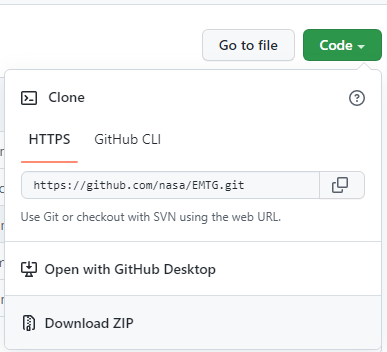
\includegraphics[width=0.5\linewidth]{../../../shared_latex_inputs/images/emtg_github_code_download.png}
			\caption{GitHub Download Prompt}
		\end{figure}
	\begin{enumerate}
		\item The user should save this directory to their local machine into a destination with no spaces in the file path and record its location for future use (e.g. C:\textbackslash SW\_Installs\textbackslash EMTG).
	\end{enumerate}
	\item Locate the folder that contains the ‘EMTG-Config-template.cmake’ file. \\ For the remainder of this document, this folder will be identified as \textbf{\textless EMTG\_root\_dir\textgreater}	
\end{enumerate}

%%%%%%%%%%%%%%%%%%%%%%%%
\section{Installing Dependencies}
\label{sec:obtaining_dependencies}
%%%%%%%%%%%%%%%%%%%%%%%%


%%%%%%%%%%%%%%%%%%%%%%%%
\subsection{Random-Number Utilities}
\label{sec:randutils}
%%%%%%%%%%%%%%%%%%%%%%%%

%%%%%%%%%%%%%%%%%%%%%%%%
% Rand utils
%%%%%%%%%%%%%%%%%%%%%%%%

\subsubsection{Purpose}
\ac{EMTG} depends on randutils for random number generation. \\ \ac{EMTG} is known to work with \hl{revision 2 of randutils}.

\subsubsection{Bundled Installation Instructions}

\begin{enumerate}
	\item Confirm the \textless EMTG-root\textgreater \textbackslash src\textbackslash Math\textbackslash randutils.hpp \hspace{1pt} file exists
	\item If the file exists, no further action is needed and you can go to the next dependency section. If for some reason the file does not exist, go to the next sub-section to download it.
\end{enumerate}

\subsubsection{Download Location}
\noindent The main page for the software distributions is in the following website: \\
\url{https://gist.github.com/imneme/540829265469e673d045}

\noindent The software revision needed for the EMTG version indicated in this guide can be obtained from the following location: \\
\emph{(In the event the url is no longer active, navigate to the aforementioned software website to find the specific version)} \\
\url{https://gist.github.com/imneme/540829265469e673d045/8486a610a954a8248c12485fb4cfc390a5f5f854}

\subsubsection{Dependency Installation Instructions}
\begin{enumerate}
	\item Click the last link in the ‘Download Location’ section
	\item Click the ‘Raw’ button
	\item Save the file to the \textless EMTG-root\textgreater \textbackslash emtg\textbackslash src\textbackslash Math\textbackslash \hspace{1pt} directory
\end{enumerate}

%%%%%%%%%%%%%%%%%%%%%%%%
\subsection{Python}
\label{sec:python}
%%%%%%%%%%%%%%%%%%%%%%%%

%%%%%%%%%%%%%%%%%%%%%%%%
% Python 
%%%%%%%%%%%%%%%%%%%%%%%%

\subsubsection{Purpose}
\noindent \ac{EMTG} depends on the Python interpreter and several packages to execute the PyEMTG \ac{GUI} and other PyEMTG utilities. PyEMTG is known to be compatible with \hl{Python 3.7}.\footnote{PyEMTG is known to specifically \emph{not} be compatible with Python 3.10 because wxWidgets is not compatible with Python 3.10.} Therefore, it is strongly recommended that a Python 3.7 environment be created for PyEMTG. There are multiple ways to get Python but we strongly recommend/support Mambaforge. The intstructions in this guide will show a user how to install Python, a user with a preexisting Python install and knowledge on using the correct environments can utilize their own Python install.

\subsubsection{Download Location}
\noindent The main page for the software distributions is in the following website: \\
\url{https://github.com/conda-forge/miniforge/}

\noindent The software package needed for the EMTG version indicated in this guide can be obtained from the following location: \\
\emph{(In the event the url is no longer active, navigate to the aforementioned software website to find the specific version)} \\
\url{https://github.com/conda-forge/miniforge/releases/tag/22.9.0-2/}

\noindent Instructions are given for creating an appropriate Python environment using the Mamba package manager. Information on obtaining and using Mamba is available at \url{https://mamba.readthedocs.io/en/latest/#}. 

\subsubsection{Dependency Installation Instructions}
\begin{enumerate}
	\item Download the Mambaforge-22.9.0-2-Windows-x86\_64.exe installer and install locally. \\ \emph{This is the installer with just mamba as the base environment}
	\item During installation, install mambaforge so it is installed just for the user. \\ See the image below for the Windows example of settings to select. 
		\begin{figure}[H]
			\centering
			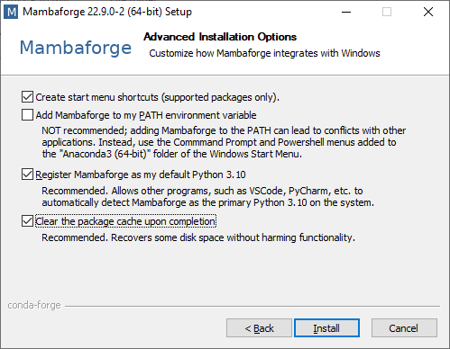
\includegraphics[width=0.5\linewidth]{../../../shared_latex_inputs/images/mambaforge_options.png}
			\caption{Mambaforge Installation Configuration}
		\end{figure}
	\item Open the MiniForge Prompt 
		\begin{figure}[H]
			\centering
			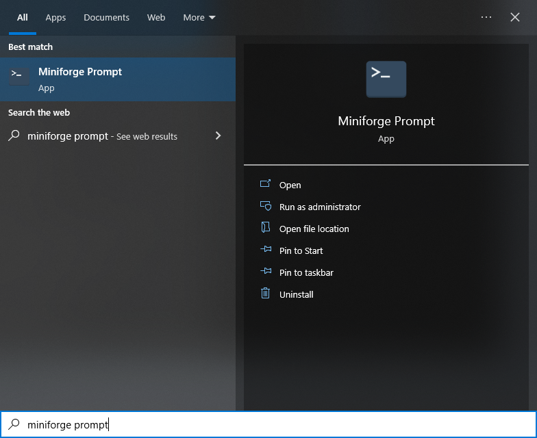
\includegraphics[width=0.5\linewidth]{../../../shared_latex_inputs/images/mambaforge_launch.png}
			\caption{Open Mambaforge Command Prompt}
		\end{figure}
	\item Type the following command and press enter to create the specific python environment for EMTG: \\ 
	\begin{verbatim}
	mamba create -n PyEmtgEnv python=3.7
	\end{verbatim}
	\begin{enumerate}
		\item Accept changes when prompted
	\end{enumerate}
	\item Type the following command and press enter to switch to the new python environment: \\ 
	\begin{verbatim}
		mamba activate PyEmtgEnv
	\end{verbatim}
	\item Enter the following to confirm the python version selected is active: \\
	\begin{verbatim}
		python --version
	\end{verbatim}	
	\item Install the following python packages
	\begin{itemize}
		\item numpy 1.21.6
		\item spiceypy 5.0.1
		\item jplephem 2.17
		\item scipy 1.7.3
		\item matplotlib 3.5.2
		\item wxPython 4.1.1
		\item astropy 4.3.1
		\item pandas 1.3.5
	\end{itemize}
	\begin{enumerate}
		\item The following is the command to use to install the various package versions listed above:\\
		\begin{verbatim}
			pip install packageName==#.#.#
		\end{verbatim}
		\item Here is an example of the command for numpy:
		\begin{verbatim}
			pip install numpy==1.21.6
		\end{verbatim}
	\end{enumerate}
	\item Enter the following to verify the stated versions of the packages were installed: \\
	\begin{verbatim}
		pip list
	\end{verbatim}	
\end{enumerate}


%%%%%%%%%%%%%%%%%%%%%%%%
\subsection{MinGW}
\label{sec:mingw}
%%%%%%%%%%%%%%%%%%%%%%%%

%%%%%%%%%%%%%%%%%%%%%%%%
% MinGW
%%%%%%%%%%%%%%%%%%%%%%%%

\subsubsection{Purpose}
\noindent \ac{EMTG} depends on the \ac{SNOPT} \ac{NLP} solver package, which is written in Fortran, and MinGW provides a free Fortran compiler and runtime library for Windows. These instructions assume that MinGW is used to compile the \ac{SNOPT} library used by \ac{EMTG}. \\ \ac{EMTG} is known to work with \hl{MinGW 7.2.0}.

\subsubsection{Download Location}
\noindent The main page for the software distributions is in the following website: \\
\url{https://sourceforge.net/projects/mingw-w64/files/}

\noindent The software package needed for the EMTG version indicated in this guide can be obtained from the following location:
\emph{(In the event the url is no longer active, navigate to the aforementioned software website to find the specific version)} \\ \url{https://sourceforge.net/projects/mingw-w64/files/Toolchains%20targetting%20Win64/Personal%20Builds/mingw-builds/7.2.0/threads-posix/seh/x86_64-7.2.0-release-posix-seh-rt_v5-rev1.7z/download}

\subsubsection{Dependency Installation Instructions}
\label{sec:mingw_installation_instructions}
\begin{enumerate}
	\item Unzip the file downloaded into a desired folder location for later use in an upcoming step. 
	\begin{enumerate}
		\item Install 7zip if that is not already installed on your machine to extract the *.7z file. 
	\end{enumerate}	
	\item Edit the user’s Path environment variable to include the bin directory of MinGW so that the EMTG executable can find the Fortran runtime library during execution.
	\begin{enumerate}
		\item Press the Windows button.
		\item Type “Edit environment variables for your account”. %\\ \emph{(Autocomplete may take over at some point.)} 
		\begin{figure}[H]
			\centering
			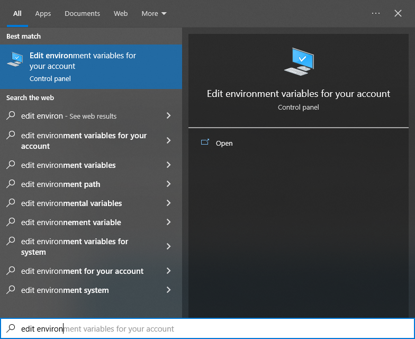
\includegraphics[width=0.7\linewidth]{../../../shared_latex_inputs/images/windows_env-variables_launch.png}
			\caption{Launching Windows Environment Variables Menu}
		\end{figure}
		\item In the upper block of the new window, labeled “User variables for [User]”, click on “Path”, then click on the “Edit...” button. 
		\begin{figure}[H]
			\centering
			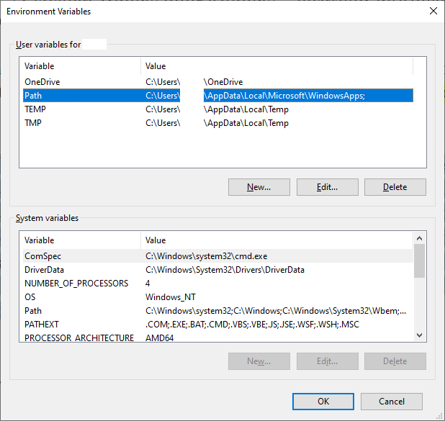
\includegraphics[width=0.7\linewidth]{../../../shared_latex_inputs/images/windows_env-variables_menu.png}
			\caption{Windows Environment Variables Menu}
		\end{figure}
		\item In the popup window, click “New”. In the new line, type the full path to the MinGW bin directory. 
		\begin{figure}[H]
			\centering
			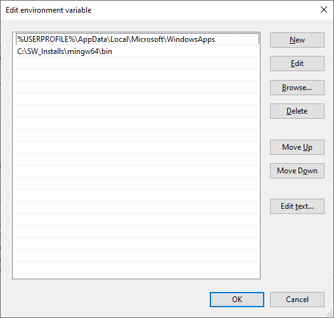
\includegraphics[width=0.7\linewidth]{../../../shared_latex_inputs/images/windows_env-variables_path.png}
			\caption{Windows Edit Environment Variable Menu}
		\end{figure}
		An example of the MinGW path would be 
		\begin{verbatim}
			C:\SW_Installs\mingw64\bin
		\end{verbatim}
		\item Click the OK button in both dialog windows to save the edit to the Path.
	\end{enumerate}		
\end{enumerate}



%%%%%%%%%%%%%%%%%%%%%%%%
\subsection{Microsoft Visual Studio}
\label{sec:visual_studio}
%%%%%%%%%%%%%%%%%%%%%%%%

%%%%%%%%%%%%%%%%%%%%%%%%
% Microsoft Visual Studio
%%%%%%%%%%%%%%%%%%%%%%%%

\subsubsection{Purpose}
\noindent \ac{EMTG} depends on a compiler to generate an executable from the source code that will function on a user's machine. \ac{EMTG} is known to work with \hl{Microsoft Visual Studio 2022 Community Edition} and this will be utilized throughout this guide. Alternative compilers can be used for users skilled enough to adapt the instructions in this guide for their compiler of choice.

\subsubsection{Download Location}
\noindent The main page for the software distributions is in the following website: \\
\url{https://visualstudio.microsoft.com/vs/community/}

\noindent The software package needed for the EMTG version indicated in this guide can be obtained from the following location: \\
\emph{(In the event the url is no longer active, navigate to the aforementioned software website to find the specific version)} \\
\url{https://visualstudio.microsoft.com/thank-you-downloading-visual-studio/?sku=Community&channel=Release&version=VS2022&source=VSFeaturesPage&passive=true&tailored=cplus&cid=2031#cplusplus}. 

\noindent \hl{Executing the Visual Studio installer requires elevated privileges.}

\subsubsection{Dependency Installation Instructions}
\begin{enumerate}
	\item Execute the downloaded file and proceed through the install instructions utilizing the defaults unless otherwise indicated in the following steps
	\item Open Visual Studio once the installer completes
	\item Follow the prompts until you reach the ‘Get started’ prompt 
		\begin{figure}[H]
			\centering
			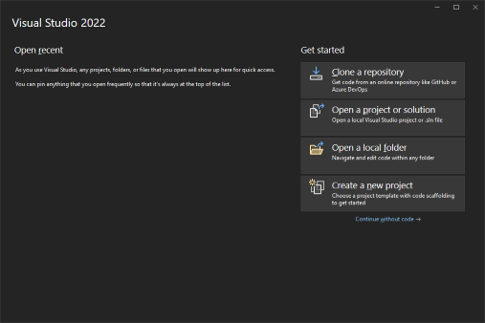
\includegraphics[width=0.9\linewidth]{../../../shared_latex_inputs/images/vstudio_init-menu.png}
			\caption{Visual Studios Startup Prompt}
		\end{figure}
	\item Click the “Continue without code” link
	\item Select ‘Tools’ -\textgreater  ‘Get Tools and Features ...’ in the tool menu
	\item Select the “Desktop development with C++” Workload
	\begin{enumerate}
		\item The selection of any other Workload and optional components is at the user's discretion
			\begin{figure}[H]
				\centering
				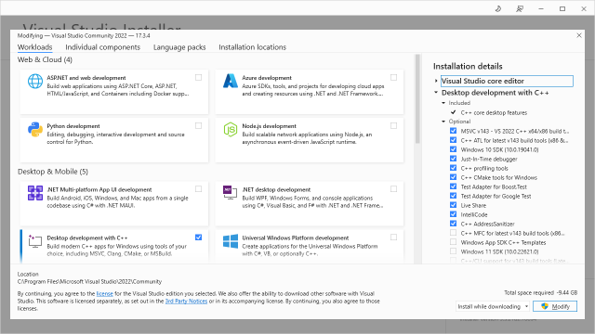
\includegraphics[width=0.95\linewidth]{../../../shared_latex_inputs/images/vstudio_cplusplus_menu.png}
				\caption{Visual Studios C++ Workload Selection}
			\end{figure}
	\end{enumerate}	
	\item Click the ‘Modify’ button, then continue through the prompts to complete the installation options needed for the remainder of the EMTG install steps
\end{enumerate}



%%%%%%%%%%%%%%%%%%%%%%%%
\subsection{CMake}
\label{sec:cmake}
%%%%%%%%%%%%%%%%%%%%%%%%

%%%%%%%%%%%%%%%%%%%%%%%%
% CMake
%%%%%%%%%%%%%%%%%%%%%%%%

\subsubsection{Purpose}
\noindent \ac{EMTG} depends on a CMake-based build system to support the generation of the executable, in addition to a compiler. \\ \ac{EMTG} is known to work with \hl{CMake 3.23.1}.

\subsubsection{Download Location}
\noindent The main page for the software distributions is in the following website: \\
\url{https://cmake.org/download/}

\noindent The software package needed for the EMTG version indicated in this guide can be obtained from the following location: \\
\emph{(In the event the url is no longer active, navigate to the aforementioned software website to find the specific version)} \\
\url{https://github.com/Kitware/CMake/releases/download/v3.23.1/cmake-3.23.1-windows-x86_64.zip}

\subsubsection{Dependency Installation Instructions}
\begin{enumerate}
	\item Extract the zip into a destination with no spaces in the file path and record its location for future use (e.g. C:\textbackslash SW\_Installs\textbackslash cmake)
	\item Navigate to the cmake ‘/bin/’ directory
	\item Right click the “cmake-gui.exe” file and select ‘Pin to Start’ to easily find the application for later use
\end{enumerate}


%%%%%%%%%%%%%%%%%%%%%%%%
\subsection{Boost}
\label{sec:boost}
%%%%%%%%%%%%%%%%%%%%%%%%

%%%%%%%%%%%%%%%%%%%%%%%%
% Boost
%%%%%%%%%%%%%%%%%%%%%%%%

\subsubsection{Purpose}
\noindent \ac{EMTG} depends on three components of Boost: filesystem, serialization, and system (and their dependencies). In addition, if a user wishes to build the \ac{EMTG} PyHardware and Propulator components, then the python component of Boost is required. \\ \ac{EMTG} is known to work with \hl{Boost 1.79.0}.

\subsubsection{Download Location}
\noindent The main page for the software distributions is in the following website: \\
\url{https://www.boost.org/users/download/}

\noindent The software package needed for the EMTG version indicated in this guide can be obtained from the following location: \\
\emph{(In the event the url is no longer active, navigate to the aforementioned software website to find the specific version)} \\
\url{https://sourceforge.net/projects/boost/files/boost-binaries/1.79.0/boost_1_79_0-msvc-14.3-64.exe/download/}

\noindent \hl{Executing the Boost installer requires elevated privileges.}

\subsubsection{Dependency Installation Instructions}
\begin{enumerate}
	\item Execute the downloaded file and proceed through the install instructions utilizing the defaults unless otherwise indicated in the following steps 
	\begin{enumerate}
		\item When prompted for the install location, save to a destination with no spaces in the file path (e.g. C:\textbackslash SW\_Installs\textbackslash boost\_1\_79\_0) and record its location for future use
	\end{enumerate}
	\item Creation of a “user-config.jam” file in your home directory
	\begin{enumerate}
		\item Navigate to your user directory (e.g. “C:\textbackslash Users\textbackslash MyName\textbackslash”)
		\item Create a “user-config.jam” file
		\item Copy the following contents to the file: \\
		\begin{verbatim}
			using python : 3.7 ; 
			using python : : C:\\Path\\To\\python.exe ;
		\end{verbatim}	
		\item 
			Replace ``\texttt{C:\textbackslash Path\textbackslash To\textbackslash python.exe}'' with the PyEmtgEnv environment that 
			contains the python 3.7 executable then save the file \\
			(e.g. \texttt{C:\textbackslash Users\textbackslash MyName\textbackslash mambaforge\textbackslash envs\textbackslash PyEmtgEnv\textbackslash python.exe})
		\\ \\
		Note that the white space is important! \\ For additional information, see the Boost documentation at \url{https://www.boost.org/doc/libs/1_79_0/libs/python/doc/html/building/configuring_boost_build.html}.
	\end{enumerate}	
	\item Open a Visual Studio Developer Command Prompt 
		\begin{figure}[H]
			\centering
			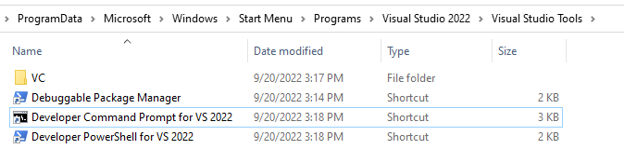
\includegraphics[width=0.9\linewidth]{../../../shared_latex_inputs/images/vstudio_cprompt_launch.png}
			\caption{Visual Studio Command Prompt Launch Icon}
		\end{figure}
	\begin{enumerate}
		\item Click the Start menu button
		\item Click on the `Visual Studio *' folder 
		\item Select the `Developer Command Prompt *' option
	\end{enumerate}
	\item Navigate to the root Boost directory (e.g. C: \textbackslash SW\_Installs \textbackslash boost\_1\_79\_0) in the command window
	\item Type the following and hit Enter:
	\begin{verbatim}
		bootstrap
	\end{verbatim}	
	\item Type the following, all on one line, and hit Enter:
	\begin{verbatim}
		.\b2 address-model=64 link=static threading=multi runtime-link=shared 
		
		--with-filesystem --with-serialization --with-system --with-python
	\end{verbatim} \\ \\
	If successful, the Boost root directory should now contain the directory path stage\textbackslash lib\textbackslash, and there should be several .lib files there. 
	\begin{figure}[H]
		\centering
		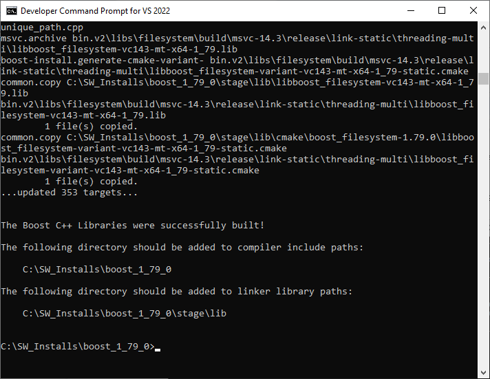
\includegraphics[width=0.7\linewidth]{../../../shared_latex_inputs/images/boost_build_success.png}
		\caption{Boost Successful Build Output}
	\end{figure}
\end{enumerate}


%%%%%%%%%%%%%%%%%%%%%%%%
\subsection{GSL}
\label{sec:gsl}
%%%%%%%%%%%%%%%%%%%%%%%%

%%%%%%%%%%%%%%%%%%%%%%%%
% GSL
%%%%%%%%%%%%%%%%%%%%%%%%

\subsubsection{Purpose}
\noindent \ac{EMTG} depends on \ac{GSL} for cubic-splining utilities. \\ \ac{EMTG} is known to work with \hl{GSL 2.4.0}. 

\subsubsection{Bundled Installation Instructions}
\begin{enumerate}
	\item Open the \textless EMTG-root\textgreater \textbackslash depend\textbackslash gsl directory.
	\item Confirm that the sub-directories contain files.
	\item If the files exist, no further action is needed and you can go to the next dependency section. If for some reason the files do not exist, go to the next sub-section to download it.
\end{enumerate}

\subsubsection{Download Location}
\noindent The main page for the software distributions is in the following website: \\
\begin{itemize}
	\item \url{https://www.gnu.org/software/gsl/#downloading}
	\item \url{https://github.com/ampl/gsl/}
\end{itemize}
	
\noindent The software revision needed for the EMTG version indicated in this guide can be obtained from the following location: \\
\emph{(In the event the url is no longer active, navigate to the aforementioned software website to find the specific version)} \\
\url{https://github.com/ampl/gsl/tree/v2.4.0}

\subsubsection{Dependency Installation Instructions}
\label{sec:gsl_installation_instructions}
\begin{enumerate}
	\item Download the zip file from the GitHub page by clicking the ‘Code’ button, select the ‘Download Zip’ option, and save to your desired location.
	\begin{figure}[H]
		\centering
		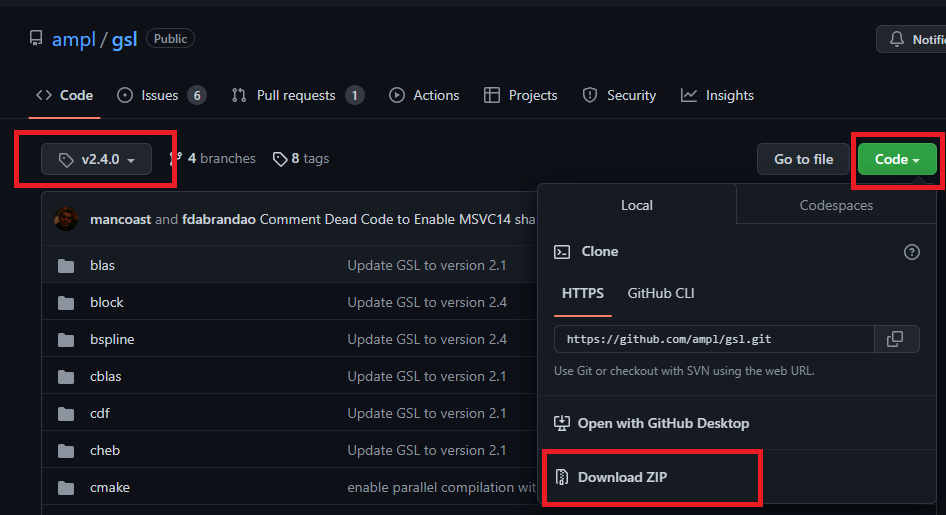
\includegraphics[width=0.9\textwidth]{../../../shared_latex_inputs/images/gsl_github.png}
		\caption{GSL Github}
	\end{figure}
	\begin{enumerate}
		\item Extract the contents of the zip file into a destination with no spaces in the file path (e.g. C:\textbackslash SW\_Installs\textbackslash gsl-2.4.0) and record its location for future use.
	\end{enumerate}
	\item \label{bundle:gsl} Open the CMake \ac{GUI}
	\item Set the CMake settings
	\begin{enumerate}
		\item Make sure that the “Advanced” and “Grouped” check boxes are checked. \\ \emph{This makes it easier to see all options}
		\item In the “Where to build the binaries:” text box, put Path/To/gsl/build. \\ It is OK if the “build” directory does not exist yet; CMake will create it. 
		\item In the “Where is the source code:” text box, put Path/To/gsl
		\item Click the ‘Configure’ button and create the build directory if prompted 
			\begin{figure}[H]
				\centering
				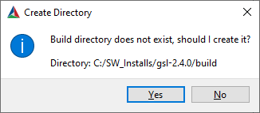
\includegraphics[width=0.5\linewidth]{../../../shared_latex_inputs/images/gsl_build_new-dir.png}
				\caption{GSL Create New Build Directory}
			\end{figure}
			\begin{figure}[H]
				\centering
				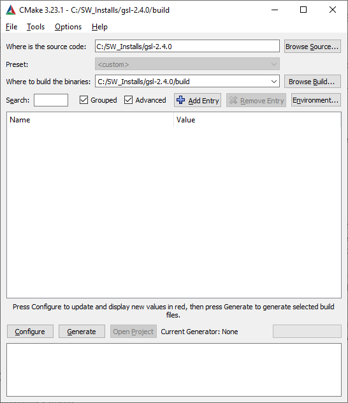
\includegraphics[width=0.7\linewidth]{../../../shared_latex_inputs/images/gsl_cmake_menu.png}
				\caption{GSL CMake Menu}
			\end{figure}
		\item If this is the first time the ‘Configure’ button has been clicked since the cache has been cleared, a popup window asking which Toolset to use will appear. Select the correct Visual Studio installation. Make sure that the “x64” toolchain is selected. \\ This pop-up can also appear on clicking the ‘Generate’ button if the cache has been cleared.
		\begin{enumerate}
			\item Verify that the “Configuring done” text is displayed in the log window
			\begin{figure}[H]
				\centering
				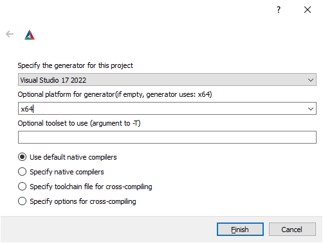
\includegraphics[width=0.7\linewidth]{../../../shared_latex_inputs/images/cmake_vstudio_select.png}
				\caption{CMake Visual Studio Settings}
			\end{figure}
		\end{enumerate}
	\end{enumerate}	
	\item Click the ‘Generate’ button
	\begin{enumerate}
		\item Verify that the “Generating done” text is displayed in the log window
	\end{enumerate}	
	\item Click the ‘Open Project’ button in the CMake GUI to open the project in Visual Studio.
	\begin{enumerate}
		\item Right-click on ‘ALL BUILD’ in the Solution Explorer pane and select the ‘Set As Startup Project’ option. 
			\begin{figure}[H]
				\centering
				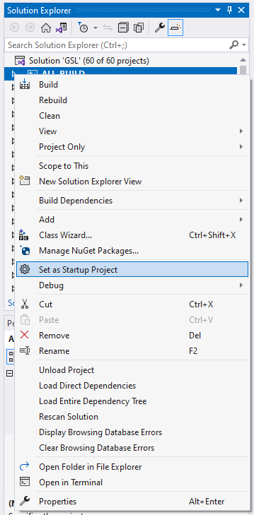
\includegraphics[width=0.35\linewidth]{../../../shared_latex_inputs/images/vstudio_set-startup.png}
				\caption{Visual Studio Select Startup Project}
			\end{figure}
		\item In the toolbar, select the ‘Release’ option from the 'Solution Configurations' dropdown.
			\begin{figure}[H]
				\centering
				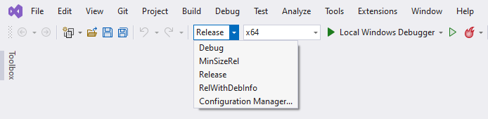
\includegraphics[width=0.7\linewidth]{../../../shared_latex_inputs/images/vstudio_config_release.png}
				\caption{Visual Studio Release Solution Configuration}
			\end{figure}
		\item Right-click on ‘ALL BUILD’ in the Solution Explorer then select the ‘Build’ option.
		\begin{enumerate}
			\item A successful build will result in a message that says, in part, “0 failed” in the Visual Studio output window. 
			\begin{figure}[H]
				\centering
				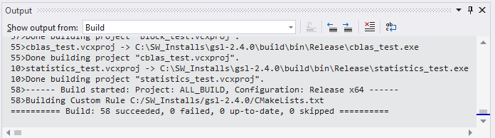
\includegraphics[width=0.7\linewidth]{../../../shared_latex_inputs/images/vstudio_gsl_success.png}
				\caption{GSL Visual Studio Success Output}
			\end{figure}
			\item The header files will be in Path/To/gsl/build/gsl.
			\item The library files will be in Path/To/gsl/build/Release.
		\end{enumerate}
	\end{enumerate}		
\end{enumerate}

%%%%%%%%%%%%%%%%%%%%%%%%
\subsection{CSPICE}
\label{sec:cspice}
%%%%%%%%%%%%%%%%%%%%%%%%

%%%%%%%%%%%%%%%%%%%%%%%%
% CSPICE
%%%%%%%%%%%%%%%%%%%%%%%%

\subsubsection{Purpose}
\noindent \ac{EMTG} depends on CSPICE for ephemeris-lookup utilities. \\ \ac{EMTG} is known to work with \hl{CSPICE N0067}. 

\subsubsection{Bundled Installation Instructions}
\begin{enumerate}
	\item Open the \textless EMTG-root\textgreater \textbackslash depend\textbackslash cspice directory.
	\item Confirm that the sub-directories contain files.
	\item If the files exist, no further action is needed and you can go to the next dependency section. If for some reason the files do not exist, go to the next sub-section to download it.
\end{enumerate}

\subsubsection{Download Location}
\noindent The main page for the software distributions is in the following website: \\
\url{https://naif.jpl.nasa.gov/naif/toolkit_C.html} 


\noindent The software revision needed for the EMTG version indicated in this guide can be obtained from the following location: \\
\emph{(In the event the url is no longer active, navigate to the aforementioned software website to find the specific version)} \\
%\url{https://naif.jpl.nasa.gov/pub/naif/toolkit//C/PC_Windows_VisualC_64bit/packages/cspice.zip}

\subsubsection{Dependency Installation Instructions}
\begin{enumerate}
	\item Once the zip file is downloaded, extract the contents of the zip file to a local folder with no space in the file path (e.g. C:\textbackslash SW\_Installs\textbackslash cspice) for usage later in these instructions.
	\item In addition to the CSPICE toolkit itself, EMTG requires ephemeris files that can be read by CSPICE. In order to get started with EMTG as quickly as possible, it is recommended to download a few commonly required ephemeris files now.
	\begin{enumerate}
		\item Navigate to \url{https://naif.jpl.nasa.gov/pub/naif/generic_kernels/spk/planets/} and download the de430.bsp file to the \textbf{\textless EMTG\_root\_dir\textgreater}\textbackslash Universe\textbackslash ephemeris\_files\textbackslash \hspace{1pt} folder
		\item Navigate to \url{https://naif.jpl.nasa.gov/pub/naif/generic_kernels/lsk/} and download the naif0012.tls file to the \textbf{\textless EMTG\_root\_dir\textgreater}\textbackslash Universe\textbackslash ephemeris\_files\textbackslash \hspace{1pt} folder
		\item Navigate to \url{https://naif.jpl.nasa.gov/pub/naif/generic_kernels/pck/} and download the pck00010.tpc and pck00011.tpc files to the \\ \textbf{\textless EMTG\_root\_dir\textgreater}\textbackslash Universe\textbackslash ephemeris\_files\textbackslash \hspace{1pt} folder
	\end{enumerate}
\end{enumerate}


%%%%%%%%%%%%%%%%%%%%%%%%
\subsection{SNOPT}
\label{sec:snopt}
%%%%%%%%%%%%%%%%%%%%%%%%

%%%%%%%%%%%%%%%%%%%%%%%%
% SNOPT
%%%%%%%%%%%%%%%%%%%%%%%%

\subsubsection{Purpose}
\noindent \ac{EMTG} depends on the commercial \ac{NLP} solver package \ac{SNOPT} to perform gradient-based optimization. \ac{EMTG} has interfaces known to work for \ac{SNOPT} versions 7.5, 7.6, and 7.7. These instructions assume that the user uses MinGW and specifically the gfortran module it is bundled with to compile \ac{SNOPT}.

\subsubsection{Download Location}
\noindent The main page for the software distributions is in the following website: \\
For more information on obtaining \ac{SNOPT}, see \url{http://www.sbsi-sol-optimize.com/asp/sol_product_snopt.htm}.

\noindent The SNOPT source code that is obtained from SBSI can be extracted to a folder on your local system. The root directory of this folder will be called \textbf{\textless SNOPT\_root\_dir\textgreater} for future references.



%%%%%%%%%%%%%%%%%%%%%%%%
% SNOPT Windows Compile Instructions
%%%%%%%%%%%%%%%%%%%%%%%%

\subsubsection{Dependency Installation Instructions}
The EMTG repository comes with sets of SNOPT CMake files for compilation of SNOPT in Windows. The following steps walk through the SNOPT compilation process using CMake.
\begin{enumerate}
	
	\item Navigate to the \textbf{\textless EMTG\_root\_dir\textgreater}\verb|\SNOPT\| directory.
	\item Copy the \verb|CMakeLists__SNOPT7-7.txt| file appropriate for your version of SNOPT and paste it into the \textbf{\textless SNOPT\_root\_dir\textgreater} directory changing the name of the file to \verb|CMakeLists.txt|.
	
	\item Navigate to the \textbf{\textless EMTG\_root\_dir\textgreater}\verb|\SNOPT\src\| directory.
	\item Copy the \verb|CMakeLists_SNOPT7-7.txt| file appropriate for your version of SNOPT and paste it into the \textbf{\textless SNOPT\_root\_dir\textgreater}\verb|\src\| directory changing the name of the file to \verb|CMakeLists.txt|.

	\item Open the \textbf{\textless SNOPT\_root\_dir\textgreater}\verb|\src\sn87sopt.f| file in a text editor
		\begin{enumerate}
			\item Navigate to approximately line 2791 for SNOPT 7.7 (line 2709 in SNOPT 7.6) and comment (Fortran uses the ! character for comments) out the line that reads 
				\begin{verbatim}
					primalInf = primalInf/max(xNorm , one)
				\end{verbatim}
			\emph{Leaving this line uncommented can incorrectly mark certain solutions as feasible in \ac{SNOPT}.}
			\item Save and close the file
		\end{enumerate}
	\item \emph{SKIP THIS STEP FOR SNOPT 7.7. This change is only required for SNOPT 7.6}\\ Open the \textbf{\textless SNOPT\_root\_dir\textgreater}\verb|\src\sn70nobj.f| file in a text editor.
		\begin{enumerate}
			\item Navigate to approximately line 235
			\item Replace the following line ...
				\begin{verbatim}
					call dload ( nF, zero, Elem, 1 )
				\end{verbatim}
				... with ...
				\begin{verbatim}
					call iload ( nF, 0, Elem, 1 )
				\end{verbatim}
				\emph{The original line could cause an error when attempting to build \ac{SNOPT} in Windows using the MinGW console as opposed to using the CMake and Visual Studio method.} 
			\item Save and close the file
		\end{enumerate}

    \item Ensure the Windows Path environment variable contains the path to the MinGW bin directory and save changes. 
	\emph{It is recommended that this be placed at or near the top of the list of directories in path. Refer to the MinGW section for additional detail.}

    \item Open the CMake GUI
	\item Set “Where is the source code” to the \textbf{\textless SNOPT\_root\_dir\textgreater} directory
	\item Set “Where to build the binaries” to \textbf{\textless SNOPT\_root\_dir\textgreater}\textbackslash build\textbackslash \\ \emph{It is OK if the ``build'' directory does not exist yet; CMake will create it.}
    \item Click ``Configure'' and make sure you are using Visual Studio 2022 toolchain and x64 which should be the CMake default. \\
	\emph{The MINGW\_GFORTRAN CMake variable should be the GFortran executable in your MinGW bin directory. Sometimes the log can say a Fortran compiler was not found but as long as the The MINGW\_GFORTRAN CMake variable shows the correct gfortran executable it is fine. If the Intel Fortran compiler, or something other than GFortran is shown here, the build will likely fail. Windows will often try to default to the Intel Fortran Compiler if installed so ensure MinGW\textbackslash bin\textbackslash  is the first directory in Path and consider removing the Intel Fortran compiler directories from Path.}

    \item Click ``Generate''
    \item Click ``Open Project'' to open Visual Studio
    \item Set build mode to Release.
    
    \begin{figure}[H]
        \centering
        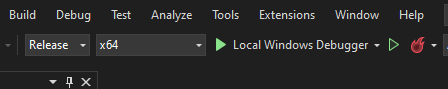
\includegraphics{../../../shared_latex_inputs/images/visual_studio_build_release.png}
        \caption{Visual Studio Build Mode}
    \end{figure}
    
    \item Build the projects in the following order: 
		\begin{itemize}	
			\item SNOPT\_build
 			\item snopt\_interface
			\item ALL\_BUILD
		\end{itemize}
    
    \begin{figure}[H]
        \centering
        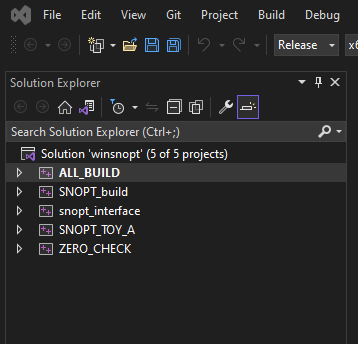
\includegraphics{../../../shared_latex_inputs/images/SNOPT_projects.png}
        \caption{Visual Studio SNOPT Solution Explorer}
    \end{figure}
    
    \item Verify the ouput window message says in part, ``0 failed, 0 skipped''. 
	The \verb|SNOPT\build\Release| directory should now look like the following image:
    
    \begin{figure}[H]
        \centering
        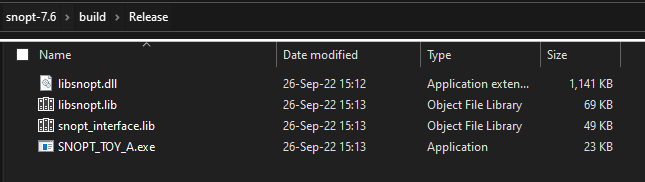
\includegraphics[width=0.9\textwidth]{../../../shared_latex_inputs/images/SNOPT_build_release.png}
        \caption{SNOPT Release Directory Contents}
    \end{figure}

\end{enumerate}



%%%%%%%%%%%%%%%%%%%%%%%%
\section{Building EMTG}
\label{sec:building_emtg}
%%%%%%%%%%%%%%%%%%%%%%%%

This section describes how to build the \ac{EMTG} executable after all dependencies have been acquired and set up. 

%%%%%%%%%%%%%%%%%%%%%%%%
\subsection{The EMTG-Config.cmake File}
\label{sec:emtg_config}
%%%%%%%%%%%%%%%%%%%%%%%%

%%%%%%%%%%%%%%%%%%%%%%%%
% 1) The EMTG-Config.cmake File
%%%%%%%%%%%%%%%%%%%%%%%%

Follow the following instructions:
\begin{enumerate}
	\item Navigate to the \textbf{\textless EMTG\_root\_dir\textgreater}\textbackslash directory
	\item Copy the `EMTG-Config-template.cmake' file and rename to `EMTG-Config.cmake'
	\item Open `EMTG-Config.cmake' in a text editor \\ \emph{This file is heavily commented with specific instructions. The user must know where they installed CSPICE, SNOPT, Boost, and GSL.}
	\item Set the CSPICE DIR variable to the full path of the CSPICE root directory.
	\begin{enumerate}
		\item If CSPICE were placed in C:\textbackslash SW\_Installs\textbackslash cspice, then the user would type in the EMTG-Config.cmake file \\
		\begin{verbatim}
			set(CSPICE_DIR C:/SW_Installs/cspice)
			 
		\end{verbatim}
		
		\emph{Note the use of forward slashes in the file path even though the Windows file system uses backslashes.}
	\end{enumerate}
	\item Set the SNOPT\_ROOT\_DIR variable to the full path of the SNOPT root directory.
	\begin{enumerate}
		\item If SNOPT  were placed in C:\textbackslash SW\_Installs\textbackslash SNOPT77, then the user would type in the EMTG-Config.cmake file \\
		\begin{verbatim}
			set(SNOPT_ROOT_DIR C:/SW_Installs/SNOPT77)
			 
		\end{verbatim}
		
		\emph{Note the use of forward slashes in the file path even though the Windows file system uses backslashes.}
	\end{enumerate}
	\item Set the BOOST\_ROOT, BOOST\_INCLUDE\_DIR, and BOOST\_LIBRARY\_DIRS variables.
	\begin{enumerate}
		\item BOOST\_ROOT is the full path to the root directory of Boost.
		\item BOOST\_INCLUDE\_DIR is the full path to the directory that contains the Boost header files. For Boost 1.79.0, this is a subdirectory in the Boost root directory called Boost.
		\item BOOST\_LIBRARY\_DIRS is the full path to the directory that holds the Boost libraries after they are built. For Boost 1.79.0, this is a subdirectory in the Boost root directory called stage\textbackslash lib.
	\end{enumerate}
	If Boost were placed in C:\textbackslash SW\_Installs\textbackslash boost\_1\_79\_0, then the user would type in the EMTG-Config.cmake file 
	\begin{verbatim}
		set(BOOST_ROOT C:/SW_Installs/boost_1_79_0) 
		set(BOOST_INCLUDE_DIR ${BOOST_ROOT}/boost) 
		set(BOOST_LIBRARY_DIRS ${BOOST_ROOT}/stage/lib) 
	\end{verbatim}	
	\emph{Note the use of forward slashes in the file path even though the Windows file system uses backslashes.}
	\item Set the GSL\_PATH variable to the full path to the GSL build directory (where the libraries are located). For example, if GSL were placed in C:\textbackslash SW\_Installs\textbackslash gsl-2.4.0, then the user would type in the EMTG-Config.cmake file 
	\begin{verbatim}
		set(GSL_PATH C:/SW_Installs/gsl-2.4.0/build)
	\end{verbatim}
	\emph{Note the use of forward slashes in the file path even though the Windows file system uses backslashes.}
	\item Save the changes made to the EMTG-Config.cmake file
\end{enumerate}

%%%%%%%%%%%%%%%%%%%%%%%%
\subsection{Setting CMake Options}
\label{sec:setting_cmake_options}
%%%%%%%%%%%%%%%%%%%%%%%%

%%%%%%%%%%%%%%%%%%%%%%%%
% 2) Setting CMake Options (Public)
%%%%%%%%%%%%%%%%%%%%%%%%

The CMake program is used to set additional options for the \ac{EMTG} build.

\begin{enumerate}
	\item Open the CMake \ac{GUI}.
	\item Make sure that the ``Advanced'' and ``Grouped'' check boxes are checked. \\ \emph{This makes it easier to see all options.}
	\item In the ``Where to build the binaries:'' text box, put \textbf{\textless EMTG\_root\_dir\textgreater}/build. \\ \emph{It is OK if the ``build'' directory does not exist yet; CMake will create it.}
	\item In the ``Where is the source code:'' text box, put \textbf{\textless EMTG\_root\_dir\textgreater}.
	\item Click ``Configure'' button.
	\item Select the options you want for each ``Name'' in the ``Value'' column. 
	\begin{enumerate}
		\item Select and confirm the appropriate SNOPT settings by following the steps below:
		\begin{enumerate}
			\item Expand the ‘Ungrouped Entries’ section
			\item Ensure SNOPT\_MINGW\_DLL is checked 
				\begin{figure}[H]
					\centering
					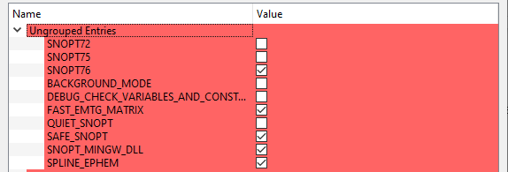
\includegraphics[width=0.7\linewidth]{../../../shared_latex_inputs/images/emtg_cmake_ungrouped-options.png}
					\caption{EMTG CMAKE Ungrouped Entries Selection}
				\end{figure}
		\end{enumerate}
		\item Ensure all the options under ``HAS'' are checked: \\ \emph{Note that for the current public release these options are not fully functional}
		\begin{enumerate}
			\item Expand the ``HAS'' section
			\item Check the HAS\_BUILT\_IN\_THRUSTERS option
			\item Check the HAS\_PROBEENTRYPHASE option 
				\begin{figure}[H]
					\centering
					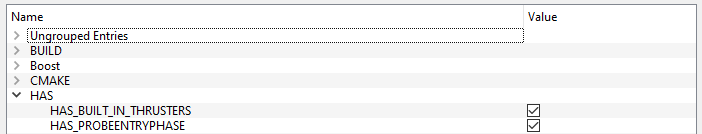
\includegraphics[width=0.75\linewidth]{../../../shared_latex_inputs/images/emtg_cmake_has-options.png}
					\caption{EMTG CMAKE Has Selection}
				\end{figure}
		\end{enumerate}
		\item Ensure Boost was detected by following the steps below:
		\begin{enumerate}
			\item Expand the ``Boost'' section
			\item Verify the directories have autopopulated to the correct location in which Boost is installed
		\end{enumerate}
		\item Enable the pyhardware and propulator utility by following the steps below:
		\begin{enumerate}
			\item Expand the ``BUILD'' section 
			\item Check the ``BUILD PROPULATOR'' option
			\item Check the ``BUILD PYHARDWARE'' option
		\end{enumerate}
	\end{enumerate}
	\item Click ``Configure''
	\item Configure the Python settings to point to the appropriate PyEMTGEnv paths:
		\begin{enumerate}
			\item Expand the ``PYTHON'' section
			\item Replace the Python paths in the PYTHON\_EXECUTABLE, PYTHON\_INCLUDE\_DIR, and PYTHON\_LIBRARY values to point to where your PyEMTGEnv is located (e.g. \verb|C:/Users/YourName/AppData/Local/mambaforge/envs/PyEmtgEnv/*|)
		\end{enumerate}
	\item Click ``Configure''
	\item Click ``Generate''
	\item Click the ``Open Project'' button \\ \emph{This will launch the Visual Studio application}
\end{enumerate}

%%%%%%%%%%%%%%%%%%%%%%%%
\subsection{Building EMTG in Visual Studio}
\label{sec:building_emtg_in_visual_studio}
%%%%%%%%%%%%%%%%%%%%%%%%

%%%%%%%%%%%%%%%%%%%%%%%%
% 3) Building EMTG in Visual Studio}
%%%%%%%%%%%%%%%%%%%%%%%%

Following the CMake configure-and-generate steps (Section~\ref{sec:setting_cmake_options}), open the project in Visual Studio. This can be done by clicking the ``Open Project'' button in the CMake \ac{GUI}. Then, perform the following actions:

\begin{enumerate}
	\item Right-click on ``EMTGv9'' in the Solution Explorer then click ``Set As Startup Project''.
		\begin{figure}[H]
			\centering
			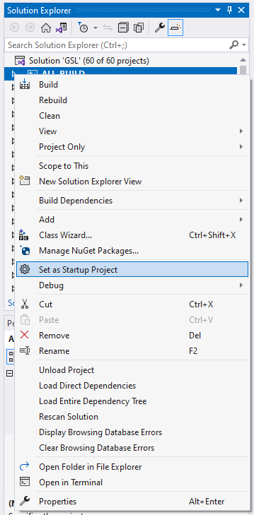
\includegraphics[width=0.35\linewidth]{../../../shared_latex_inputs/images/vstudio_set-startup.png}
			\caption{Visual Studio Select Startup Project}
		\end{figure}	
	\item In the toolbar, select the ``Release'' option from the ``Solution Configurations'' dropdown.
		\begin{figure}[H]
			\centering
			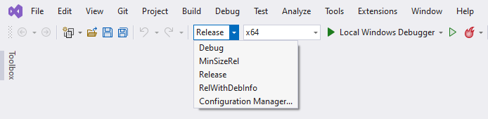
\includegraphics[width=0.7\linewidth]{../../../shared_latex_inputs/images/vstudio_config_release.png}
			\caption{Visual Studio Release Solution Configuration}
		\end{figure}
		\emph{Do not select ``Debug'' unless you actually want to debug \ac{EMTG}!}
	\item Right-click on ``EMTGv9'' in the Solution Explorer then click ``Build''.
	\item Verify the build is successful. \\ \emph{The log output will result in a message that says, in part, ``0 failed'' in the Visual Studio output window. In addition, Path/To/EMTG/Repo/bin will contain EMTGv9.exe and libsnopt.dll.}
\end{enumerate}


%%%%%%%%%%%%%%%%%%%%%%%%
\section{Executing EMTG}
\label{sec:pyemtg_look_elsewhere}
%%%%%%%%%%%%%%%%%%%%%%%%

\subsection{Using PyEMTG GUI}
%%%%%%%%%%%%%%%%%%%%%%%%
%\section{PyEMTG}
%\label{sec:pyemtg_look_elsewhere}
%%%%%%%%%%%%%%%%%%%%%%%%

PyEMTG is a set of Python scripts that provide capabilities such as a \ac{GUI} for \ac{EMTG} and automated trade study utilities (i.e., \ac{PEATSA}). Full PyEMTG documentation is contained in the \ac{EMTG} repository's /PyEMTG/docs/ directory. In that directory, see PyEMTG\_docs\_readme.pdf for an overview of available PyEMTG documentation, which includes a reference to the PyEMTG User's Guide.
%%%%%%%%%%%%%%%%%%%%%%%%
% Executing PyEMTG in Windows
%%%%%%%%%%%%%%%%%%%%%%%%

\noindent The following actions are instructions on executing PyEMTG on Windows and running the default mission:

\begin{enumerate}
	\item Navigate to the \textbf{\textless EMTG\_root\_dir\textgreater}\textbackslash PyEMTG\textbackslash \hspace{1pt} folder
	\item Copy the PyEMTG-template.options file to a new file called PyEMTG.options
	\item Open the newly copied PyEMTG.options file in a text editor
	\item Replace the ‘EMTG\_path’ value with the \textbf{\textless EMTG\_root\_dir\textgreater}/bin/EMTGv9.exe path \\ \emph{This path needs to have forward slashes (/)}
	\item Replace the ‘default\_universe\_path’ value with the \textbf{\textless EMTG\_root\_dir\textgreater}/Universe path\\ \emph{This path needs to have forward slashes (/) and do not have a trailing forward slash}
%	\item Replace the ‘default\_small\_bodies\_file’ value with the\hspace{0.5pt} \textbf{\textless EMTG\_root\_dir\textgreater}/Universe/ \\ ephemeris\_files/*.bsp asteroid file path downloaded in a previous step \\ \emph{This path needs to have forward slashes (/) and do not have a trailing forward slash}
	\item Save the PyEMTG.options file and close the text editor
	\item Navigate to the ‘Miniforge Prompt’ window where the PyEmtgEnv environment is active
	\item Type the following in the prompt, replacing \textbf{\textless EMTG\_root\_dir\textgreater} with your EMTG directory path, and press enter:
	\begin{verbatim}
		cd <EMTG_root_dir>\PyEMTG\
	\end{verbatim}
	\item Type the following in the prompt and press enter to Launch PyEMTG:
	\begin{verbatim}
		python PyEMTG.py
	\end{verbatim}
	\item Click File -\textgreater \hspace{1pt}New -\textgreater \hspace{1pt}Mission option\\ \emph{The default Mission values will be loaded.}
	\item Click on the `Spacecraft Options' tab 
	\item Click the `ellipsis' button associated with the `Hardware library path' field and select the \textbf{\textless EMTG\_root\_dir\textgreater}\textbackslash HardwareModels\textbackslash \hspace{1pt} folder and click `Select Folder'
	\item Add a `\textbackslash' \hspace{1pt} to the end of the string in the `Hardware library path' field if one is not already there
	\item Click the `ellipsis' button associated with the `Launch vehicle library file' field and select the default.emtg\_launchvehicleopt file and click `Open'
	\item Click the `Launch vehicle' dropdown and select `ExampleRocket'
	\item Click on the `Physics Options' tab 
	\item Click the `Default' button associated with the `Universe folder' field \\ \emph{This will populate the field with the value from the PyEMTG.options file.}
	\item Verify the `Leap seconds kernal' and `Frame kernel' filenames are the latest .tls and .tpc files, respectively available, in the \textbf{\textless EMTG\_root\_dir\textgreater}\textbackslash Universe\textbackslash ephemeris\_files\textbackslash \hspace{1pt} folder
	\item Click on the `Journey Options' tab 
	\item Click the `ellipsis' button associated with the `Central body' field
	\item Select the Sun\_barycenters.emtg\_universe and click the `Open' button
	\item Click File -\textgreater \hspace{1pt}Run option
	\item Rename the mission file to the name of your choosing and click the `Save' button \\ \emph{At this point, PyEMTG will execute EMTG and a new command window will open that will display the output generated from EMTG}
\end{enumerate}

\subsection{Using Command Line}
\label{sec:executing_emtg_without_pyemtg}

%%%%%%%%%%%%%%%%%%%%%%%%
%\section{Executing \ac{EMTG} Without PyEMTG}
%\label{sec:executing_emtg_without_pyemtg}
%%%%%%%%%%%%%%%%%%%%%%%%

On a local Windows machine, \ac{EMTG} is most often executed via the PyEMTG \ac{GUI}. However, it may also be executed from the command line, from a script, or using the Windows Explorer. In the first two instances, \ac{EMTG} is executed by invoking the EMTGv9.exe command with the name of an \ac{EMTG} options file (``*.emtgopt'') as the only command-line argument. To execute via Windows Explorer, open two Windows Explorer windows. In one, navigate to Path/To/EMTG/Repo/bin. In the other, navigate to the location of the \ac{EMTG} options file to be executed. Drag and drop the \ac{EMTG} options file onto EMTGv9.exe to execute.


%\bibliographystyle{AAS_publication}
%\bibliography{EMTGbib_Jacob_June_2014}


\end{document}
